% 
% Annual Cognitive Science Conference
% Sample LaTeX Paper -- Proceedings Format
% 

% Original : Ashwin Ram (ashwin@cc.gatech.edu)       04/01/1994
% Modified : Johanna Moore (jmoore@cs.pitt.edu)      03/17/1995
% Modified : David Noelle (noelle@ucsd.edu)          03/15/1996
% Modified : Pat Langley (langley@cs.stanford.edu)   01/26/1997
% Latex2e corrections by Ramin Charles Nakisa        01/28/1997 
% Modified : Tina Eliassi-Rad (eliassi@cs.wisc.edu)  01/31/1998
% Modified : Trisha Yannuzzi (trisha@ircs.upenn.edu) 12/28/1999 (in process)
% Modified : Mary Ellen Foster (M.E.Foster@ed.ac.uk) 12/11/2000
% Modified : Ken Forbus                              01/23/2004
% Modified : Eli M. Silk (esilk@pitt.edu)            05/24/2005
% Modified : Niels Taatgen (taatgen@cmu.edu)         10/24/2006
% Modified : David Noelle (dnoelle@ucmerced.edu)     11/19/2014

%% Change "letterpaper" in the following line to "a4paper" if you must.

\documentclass[10pt,letterpaper]{article}

\usepackage{hyperref}
\usepackage{cogsci}
\usepackage{pslatex}
\usepackage{amsfonts}
\usepackage{graphicx}
\usepackage{apacite}
\usepackage{color}
\usepackage{todonotes}

\definecolor{Red}{RGB}{255,0,0}
\newcommand{\red}[1]{\textcolor{Red}{#1}}

\newcommand{\jd}[1]{\green{$^*$}\marginpar{\footnotesize{JD: \green{#1}}}}

\newcommand{\subsubsubsection}[1]{{\em #1}}
\newcommand{\eref}[1]{(\ref{#1})}
\newcommand{\tableref}[1]{Table \ref{#1}}
\newcommand{\figref}[1]{Figure \ref{#1}}
\newcommand{\appref}[1]{Appendix \ref{#1}}
\newcommand{\sectionref}[1]{Section \ref{#1}}

\title{Why do you ask? To be informative.}
 
\author{{\large \bf Robert X.~D.~Hawkins (rxdh@stanford.edu)} \AND {\large \bf Andreas Stuhlm\"uller (andreas@stuhlmueller.org)}\\ 
	\AND
	{\large \bf Judith Degen (jdegen@stanford.edu)} 
  \AND {\large \bf Noah D.~Goodman (ngoodman@stanford.edu)} \\
  Department of Psychology, 450 Serra Mall \\
  Stanford, CA 94305 USA}


\begin{document}

\maketitle


\begin{abstract}


\textbf{Keywords:} 
questions; answers; computational pragmatics; theory of mind; 
\end{abstract}

\section{Introduction}
\label{sec:intro}

<<<<<<< Updated upstream
\todo[inline]{NDG: there is a lot of good stuff in the intro below, but it is not globally coherent yet. let's discuss the flow of the argument we want to make...}

\todo[inline]{NDG: this discussion of intention inference is good, but i think we should start with a few sentences more directly about questions and answers. i often like to start with an example, if there is a short and illustrative one...}
%Humans are experts at inferring the intentions of other agents from their actions \cite{TomaselloCarpenter___Moll05_IntentionsCulturalCognition}. Given simple motion cues, for example, we are able to reliably discern high-level goals such as chasing, fighting, courting, or playing \cite{BarrettToddMillerBlythe05_IntentionFromMotionCues, HeiderSimmel44_ApparentBehavior}. 
How would you respond if someone asked ``where are you?'' There are a number of valid answers at different levels of coarseness:  \emph{in the kitchen}, \emph{at home}, \emph{in Chinatown}, \emph{in San Francisco}, \emph{on Earth}, and so on. Which one do you use? The answer will depend in some way on context and, in particular, on the intentions of the questioner. If you had plans to meet a colleague at a coffee shop and you're running late, you might give a fairly specific answer to indicate you're close by. On the other hand, you might use a coarser answer if you just flew into a new city for a conference and were calling home to say that you're safe. Crucially, though, 

Experiments in psycholinguistics have shown that this expertise extends to speech acts as well. For example, when people are asked `Do you have the time?'' they typically round their answers to the nearest 5 or 10 minute interval, even when they're wearing a digital watch \cite{DerHenstCarlesSperber02_RelevanceTellingTime}. However, if the question is preceded by the statement ``My watch stopped,'' people make their response precise to the minute  \cite{GibbsBryant08_OptimalRelevance}. This demonstrates sensitivity to questioner goals, and a pragmatic imperative to maximize relevance with respect to those goals. 

Similar evidence comes from a classic study where researchers called liquor merchants and asked, ``Does a fifth of Jim Beam cost more than \$5?'' If this was preceded by the statement, "I want to buy some bourbon,'' merchants gave the actual price significantly more frequently than when it was preceded by the statement, ``I've got \$5 to spend.'' In the former case, the merchant inferred that the questioner's goal was just to buy whiskey, so the exact price is the maximally relevant response. In the latter case, the merchant inferred that the questioner's goal was literally to find out whether or not they could afford the whiskey, hence a simple `yes'  sufficed \cite{Clark79_IndirectSpeechActs}. Context and questioner goals have also been implicated in accounts of identification questions like ``who is X?'' \cite{BoerLycan75_KnowingWho}, and to questions like ``where are you?'' that permit answers at many levels of abstraction\cite{Potts12_CardsDialogueCorpus}.

\todo[inline]{NDG: i would set up the puzzle for (RSA style) models around here? say that recent formal models of pragmatics have made progress specifying the nature and role of information and goals for statements, but they have a problem when it comes to questions? then turn to other's answers?}

\red{XXX what are some useful anwers other people have given? why do we think those answers are nevertheless lacking? \textbf{Judith} XXX I describe Groenendijk and van Rooy below: any others? \textbf{Robert}}

What makes a question useful? What makes an answer to a question useful? 
In this paper, we propose an account of question and answer behavior in which the questioner's�intentions are \emph{not} known \emph{a priori} by the answerer and instead must be inferred. We propose that a useful answer to a question is one that is maximally informative with respect to this inferred underlying decision problem. A useful question, then, is one that optimally \emph{signals} the questioner's underlying decision problem and has a high probability of resulting in an answer that is maximally informative with respect to that decision problem. This places question and answer behavior in the larger class of social behavior governed by theory of mind.

The rest of this paper is structured as follows. First, we specify a family of questioner and answerer agents extending the Rational Speech Act (RSA) framework \cite{frank2012, GoodmanStuhlmuller13_KnowledgeImplicature}, highlighting some points of divergence from previous RSA models. We then individuate three particular models in this family, representing progressively more sophisticated hypotheses about how questioners and answerers reason about their task. In particular, we compare a pragmatic answerer making inferences about the questioner's goals to two simpler models: one that takes into account only that an answerer wants to be maximally informative with respect to the explicit question asked (without inferring the questioner's underlying decision problem) and one that provides a literal answer to the question (without attempting to be maximally informative). 

To compare these models, we derive predictions for a pair of experiments using a novel guessing-game task, and compare these predictions to human performance. In one phase of the task, we require participants to ask a question (from a fixed set of possible questions), given a decision problem. In the second phase, we require participants to give an answer (from a fixed set of possible answers) to a question (from a fixed set of possible questions). 

\section{A Rational Speech Act model of question and answer behavior}
\label{sec:model}

\todo[inline]{NDG: i think it will make more sense to start with the top-level cognitive models for the Q and A, and then fill down to the sub-agents as increasingly complicated notional communicative partners.}

\red{XXX Should give a couple sentences about the idea of RSA models in general before launching into our specific instantiation \textbf{Robert}}. Suppose there is a set of distinct world states $\mathcal{W}$, a set of possible goals $\mathcal{G}$, a set of possible questions $\mathcal{Q}$, and a set of possible answers $\mathcal{A}$. These sets are all taken to be in common ground. The simplest answerer model contains two agents: the literal listener, which serves as an interpreter for the meaning of question/answer pairs, and a literal answerer, who simply tries to convey the state of the world, regardless of the question.

\begin{itemize}
\item The \textbf{literal listener} takes a question utterance $q \in \mathcal{Q}$ and an answer utterance $a \in \mathcal{A}$ as input and returns a distribution over worlds in which the meaning of the answer, given the meaning of the question, is true. For example, if the questioner asked ``do you have a car?'' and the answerer responded ''yes'', the literal listener would return a distribution over worlds in which the answerer has a car. In general, the meaning function defined on $\mathcal{A}$ and $\mathcal{Q}$ depends on the task being modeled. 

\item The \textbf{literal answerer} takes a question utterance $q \in \mathcal{Q}$ and a world state $w \in \mathcal{W}$ as input and returns a distribution over the answer space $\mathcal{A}$. It samples an answer  $a$ from $\mathcal{A}$ with prior probability $P(a)$ and conditions on the likelihood of the questioner inferring the true world $w$ from this answer, by consulting the literal listener. Note that this agent ignores the question; it's only concern is to convey the true state of the world.
\end{itemize}

The literal answerer model predicts that answerer behavior will be independent of the question being asked, but will still be useful in the sense that it reduces the questioner's uncertainty about the state of the world. This is essentially the speaker model from previous RSA models. 

Next, we specify an alternative answerer, the \emph{explicit answerer}, which attempts to be informative not just with respect to the true state of the world, but  more specifically, with respect�to the \emph{aspect of the world} explicitly picked out by the question utterance:

\begin{itemize}

\item The \textbf{explicit answerer} takes a question utterance $q \in \mathcal{Q}$ and a world state $w \in \mathcal{W}$ as input and returns a distribution over the answer space $\mathcal{A}$. It samples an answer  $a$ from $\mathcal{A}$ with prior probability $P(a)$, consults the literal listener about the distribution of worlds that are consistent with this answer, and conditions on the likelihood that the feature of the world explicitly mentioned in the question $q$ is true in this distribution: $P(a | q, w) = P(q(w) | a) \times P(a)$. \red{Is this the right way to write this?}

\end{itemize}

Here, the goal of the agent is still to impart information, but unlike the literal answerer, it uses the question as a measure for weighing what pieces of information are most relevant. For example, if the questioner asked ``Do you have a car?'' the literal answerer could say all kinds of true things about the world, like ``I have a bicycle'' or ``I saw a car this morning,'' but the explicit answerer would prefer an answer that, after being filtered through the literal listener, generates a set of worlds that match the true world on the salient attribute: whether or not the answerer has a car.

For every answerer we build, we can build a corresponding questioner agent. Critically, instead of trying to impart information about the state of the world, questioners are trying to \emph{learn information about a private goal}, sometimes called a QUD (or question under discussion) \cite{Roberts96_InformationStructureDiscourse}.In order to pick which question to ask, they reason about how their internal model of an answerer would respond given some true world, and condition on the expected information gain after hearing this response, averaged across the space of possible worlds. 

\begin{itemize}

\item The \textbf{questioner} takes a goal $g \in \mathcal{G}$ as input and returns a distribution over questions $\mathcal{Q}$. It first computes a prior $P(w)$ over states of the world, weighted by their priority under the goal $g$. Next, it samples a question $q \in \mathcal{Q}$ and computes the expected information gain from hearing the answerer's response to that question. Information gain is measured as the Kullback-Leibler divergence between the prior distribution $P(w)$ and the posterior distribution over world states after conditioning on an answer: 
$$P(q | g) = \mathbb{E}_w [D_{KL}(P(w)\, \| \, P(w | a)P(a | q,w)]$$ where $P(a | q,w)$ is the response distribution returned by reasoning about what an answerer would do.

\end{itemize}

Now that we have a set of questioners defined, we can present our final model of answerer behavior: the pragmatic answerer. Instead of being informative with respect to the aspects of the world picked out by an explicit question, it reasons about the \emph{goals that may have generated} that question, and is informative with respect to these goals instead.

\begin{itemize}

\item The \textbf{pragmatic answerer} takes a question utterance $q \in \mathcal{Q}$ and a world state $w \in \mathcal{W}$ as input and returns a distribution over the answer space $\mathcal{A}$. First, it uses the questioner defined above as a generative model of questions given goals in order to estimate the likelihood of different goals given the question $q$. It samples an answer $a$ from $\mathcal{A}$ with prior probability $P(a)$, consults the literal listener about the distribution of worlds that are consistent with this answer, and conditions on the likelihood that the feature of the world \emph{picked out by the inferred goal} is true in this distribution.

\end{itemize}

This concludes our specification of the model space. Within this computational framework, different theories of question and answer behavior can be formalized and compared on the basis of their predictions. Assumptions about what is held in common ground are made transparent, and we can systematically manipulate individual elements of the model to test how they affect overall predictions. Because these are probabilistic models, we can succinctly write them down and evaluate their predictions in a probabilistic programming language \cite{Goodman13_POPL}. The model predictions shown throughout the rest of the paper were computed using a language called WebPPL \cite{GoodmanStuhlmuller14_DIPPL}. Note that this specification diverges from previous work in the RSA framework in a few key ways: (1) for the questioner, we replace the goal of imparting information with the goal of learning information about the specified QUD and (2) \dots \red{XXX there are probably other differences I can't think of \textbf{Robert}}.

\begin{figure}
\begin{center}
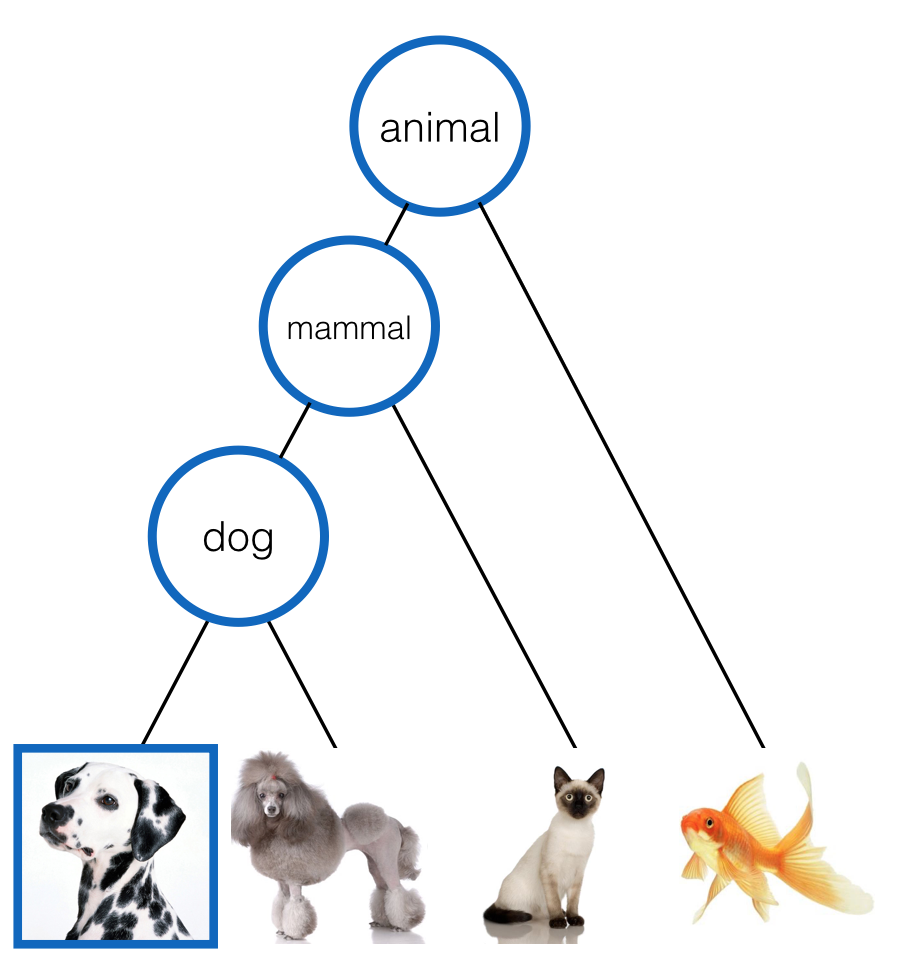
\includegraphics[scale = .2]{taskhierarchy}
\end{center}
\caption{Hierarchy of objects used in experiment 1}
\label{fig:taskhierarchy}
\end{figure}

\section{Experiment 1: \\ Questions and answers in a hierarchical world}

In order to test how questioners choose questions when given a decision problem, and how answerers choose answers under uncertainty about this decision problem, we designed a guessing-game task played by two players: a guesser and a helper. In this game, $4$ animals (a dalmatian, a poodle, a siamese cat, and a goldfish) were hidden behind $4$ gates. Note that these animals were arranged in a class hierarchy (see Fig. \ref{fig:taskhierarchy}). The guesser was given a private goal of finding one of the objects, and the helper had privileged information about the exact locations of each object. Before choosing a gate, the guesser could ask the helper a single question, and the helper could respond to this question by revealing the object behind a single gate. 

In terms of our model specification, the world space $\mathcal{W}$ is the set of $4! = 24$ possible assignments of four objects to four gates and the goal space $\mathcal{G}$ is the set of four objects that the guesser could possibly be trying to find, and the answer space $\mathcal{A}$ is the set of four gates that the helper could possibly reveal. The key constraint in the task, however, is that the guesser must choose from a \emph{restricted set of questions}: they may be trying to find the goldfish, but cannot directly ask `where is the goldfish?' Instead, the question space $\mathcal{Q}$ is the set of highlighted nodes in the hierarchy, including higher order nodes that are consistent with multiple answers. \ref{XXX Robert: Probably need to define the question meaning and answer meaning functions to make the literal listener concrete...}
\begin{figure*}[t!]
\begin{center}
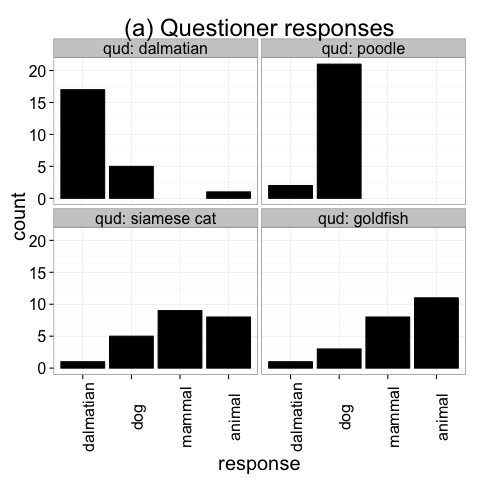
\includegraphics[scale = .5]{exp3_q}
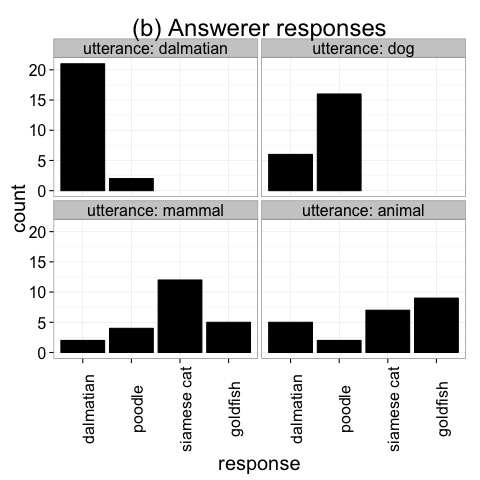
\includegraphics[scale = .5]{exp3_ans}
\end{center}
\caption{Experiment 1 results}
\label{fig:exp1res}
\end{figure*}
%\label{sec:expq}

We recruited 25 participants from Amazon Mechanical Turk to participate in this task. Each participant provided responses for four trials in the role of the questioner (corresponding to each goal in $\mathcal{G}$), and four trials in the role of the answerer (corresponding to each question in $\mathcal{Q}$). In order to collect responses for all elements of $\mathcal{G}$ and $\mathcal{Q}$, The order of� the questioner and answerer blocks was randomly assigned, and the order of stimuli within these blocks was also randomized\footnote{All materials are available on \href{https://github.com/hawkrobe/Q\_and\_A/tree/master/experiment3/versions/experiment3\_short}{Github}}. Two participants were excluded due to self-reported confusion about the task.

Results for the guesser role are shown in Figure \ref{fig:exp1res}(a). There are two primary trends to note in these data. First, questioners tend to choose the indirect question node closest to their goal when the direct question is unavailable. It is unsurprising that they ask about the `dalmatian` when looking for the dalmatian, but interesting that they strongly prefer asking about a `dog' when looking for the poodle, about a `mammal' when looking for the cat, and so on. \red{XXX need statistics here. Probably will need more than 25 participants to get enough power... \textbf{Robert}} 


Results for the helper role are shown in Figure \ref{fig:exp1res}(b). The most striking feature of these data is how closely match the questioner distribution \red{XXX Possibly just because people did both... It might be the second-timers driving the effect, so we should separate out the different orders, or run it again between-subjects \textbf{Robert}}. If the helper is asked about a `dog`, the dalmatian and poodle would be equally good literal answers to this question, but they strongly prefer to give the location of the poodle. Similarly, the dalmatian, poodle, and siamese cat are all mammals, but helpers prefer to respond to the `mammal' question by revealing the location of the cat. 

We now compare these results to the predictions of our family of models. At the very simplest level, our \emph{literal answerer} yields a uniform distribution over the four answers that are the case in the given world. This has important consequences for the corresponding questioner model: when this questioner reasons about which question would generate the most helpful answer from the literal answerer, they find no difference across questioners, and therefore have no preference over which question to ask. This is clearly not the case and we will not consider these options further.

At a slightly higher level of sophistication, we have an \emph{explicit answerer}. It up-weights answers that result in a distribution of worlds where as many as possible of the leaf nodes picked out by the question are in the correct location. Similarly, it down-weights answers that would mislead the questioner into the thinking that the leaf nodes mentioned in the question are in the wrong locations.  This model produces the answerer predictions depicted in Figure \ref{fig:exp1pred}(b), which successfully down-weights the least relevant alternatives but cannot break the symmetries between the explicitly relevant ones, and is therefore unable to satisfactorily account for our data. 

While our `explicit answerer' model cannot account for answerer data, it does provide a foundation for a reasonably well-performing questioner model. When the questioner selects questions that maximize the expected information gain of the explicit answerer's response, it produces the distribution of questions shown in Figure \ref{fig:exp1pred}(a) \dots \red{XXX Will fill in once we have better questioner predictions \textbf{Robert}}

Finally, we examine a pragmatic answerer that begins by estimating the likelihood of the questioner having a goal $g$ given the question being asked. It then applies this distribution of goals as the criterion for whether an answer is useful: it prefers answers for which the distribution of consistent worlds have the item specified by the particular goal is in the right position. The results for this answerer are depicted in Figure \ref{fig:exp1pred}(c).

%We will delay our full model evaluation until after describing a second experiment, but we suggest at this stage that some pragmatic inference appears be taking place on the part of the answerer. In discerning why the questioner would ask about the dog, they might reason as follows: `if the questioner wanted to know the location of the dalmatian, he or she would have asked about the dalmatian. They didn't, therefore, they must be interested in the other dog: the poodle.' 

To address concerns that the preceding results were due to particular features of the design such as the one-to-one mapping from goals to questions and from questions to answers, which gives the task the sense of an 'elimination game,' we ran a second experiment using a larger hierarchy \dots

\section{Experiment 2: }
\label{sec:expa}

\red{XXX TODO}

\begin{figure*}[t!]
\begin{center}
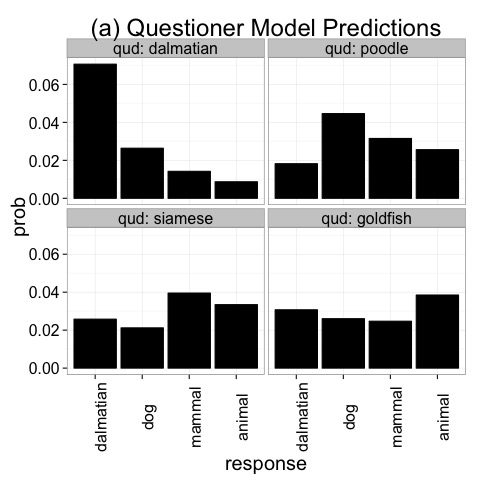
\includegraphics[scale = .33]{Exp3QuestionerPrediction}
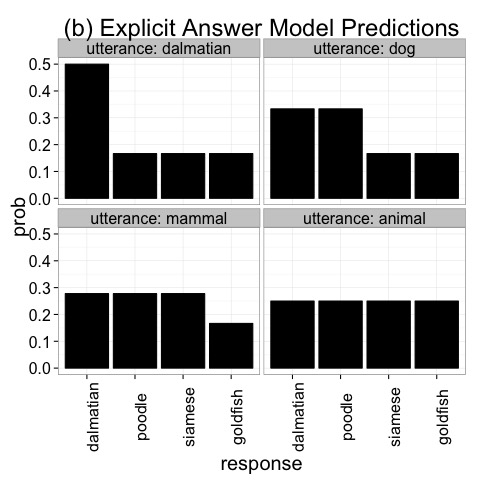
\includegraphics[scale = .33]{Exp3ExplicitAnswerPrediction}
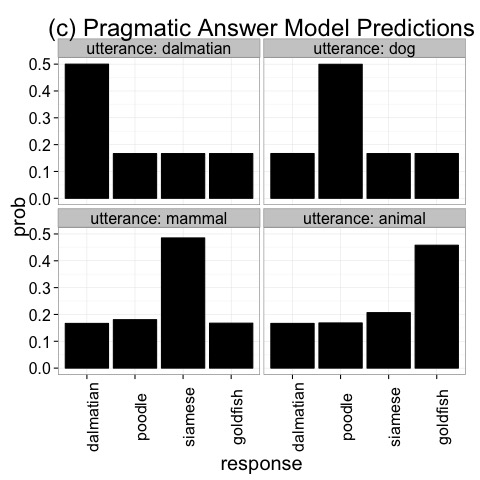
\includegraphics[scale = .33]{Exp3PragmaticAnswerPrediction}
\end{center}
\caption{Experiment 1 model predictions \red{XXX Robert: when we've got the models right and have actually fit the rationality parameter to the data, we should put a scatter plot here, or show the data and predictions side by side. This is hard to compare with the results on the previous page.} }
\label{fig:exp1pred}
\end{figure*}

\section{Related work}

Our account of question and answer behavior ultimately converges on a similar solution as contemporary decision theoretic or game theoretic accounts in linguistics. These theories were a response to early work on question and answer semantics, which focused on the notion of informativeness. In Groenendijk \& Stokhof's \citeyear{GroenendijkStokhof84_SemanticsOfQuestions} theory of question and answer semantics, asking a question induces a partition over the space of possible worlds, where each cell of the partition corresponds to a possible answer. An answer, then, consists of eliminating cells in this partition, and the most useful answers are those that eliminate all relevant alternatives to the true world. However, as van Rooy \cite{VanRooy03_QuestioningDecisionProblems} and others \cite{Ginzburg95_ResolvingQuestions} have pointed out, this predicts that \emph{wh}-questions like ``Where can I buy an Italian newspaper?'' can only be fully resolved by exhaustively mentioning whether or not such a newspaper can be bought at each possible location. Clearly, this is not the case: a single nearby location would suffice. These theories also cannot account for other contextual variation in what counts as a useful answer, such as questions like ``where are you?'' 

More recent theories have tried to fix these problems by introducing some consideration of the questioner's goals. van Rooy \citeyear{VanRooy03_QuestioningDecisionProblems}, for instance, formalizes these goals as a decision problem faced by the questioner. A useful answer under this decision theoretic account is one that maximizes the expected value of the questioner's decision problem. A useful question is one that induces a sufficiently fine-grained partition, optimally distinguishing the worlds relevant to the decision problem. While this framework elegantly accounts for the context-dependence and relevance-maximization of question and answer behavior, it assumes that the questioner's decision problem is known \emph{a priori} by the answerer. If this were the case, the act of asking questions would seem irrelevant: why wouldn't the answerer directly tell the questioner which action to take? 

\section{General discussion}
\label{sec:gd}

Behind every question lies some goal or intention. This could be an intention to obtain an explicit piece of information (``Where can I get a newspaper?''), signal some common ground (``Did you see the game last night?''), test the answerer's knowledge (``If I add these numbers together, what do I get?''), politely request the audience to take some action (``Could you pass the salt?''), or just to make open-ended small talk (``How was your weekend?''). Intuitively, these wildly different intentions seem to warrant different kinds of answers, even if the explicit question is expressed using the same words.

In this paper we have presented computational-level evidence that answerer behavior is best described by a pragmatic model that reasons about questioner intentions, using the question utterance as a signal. This analysis provides a novel perspective on the role of questions in dialogues: it is well-accepted under the Gricean view that answerers strive to be relevant, but we find that there is also a burden placed on the questioner to provide sufficient information about should be considered relevant in the first place. By artificially restricting the question space in our experiments, we have shown that when necessary, questioners can reliably choose an optimally informative signal.

\red{XXX}

\bibliographystyle{apacite}

\setlength{\bibleftmargin}{.125in}
\setlength{\bibindent}{-\bibleftmargin}

\bibliography{bibs}


\end{document}
